\chapter{Resultados}
\label{cap:Resultados}
En este capítulo se explican los resultados obtenidos en cada uno de los sprints del desarrollo del trabajo y cómo se relacionan con los objetivos definidos.

[... Hablar acerca de los hitos ...]


\section{Identificación y adquisición de las variables del sistema}
En la primera iteración se busca identificar cada una de las variables que entran en juego en el sistema, así como su proceso de obtención. Se debe tener clara la diferencia entre variables de entrada y salida y variables de control.
\subsection{Variables de entrada}
Son las fuentes de suministro de energía al sistema. Habrá un total de tres:
\begin{itemize}
	\item \textbf{Energía fotovoltaica (EF)}\\ Energía procedente de las placas solares. Su valor viene determinado por varios factores, como son el número de módulos fotovoltaicos instalados y la máxima potencia posible en cada momento, \textit{current module power} (CMP). Hace referencia a la potencia de salida, en watios que produce un panel fotovoltaico en condiciones de máxima iluminación solar, con una radiación de aproximadamente 1 kW/m2. Será dependiente de la situación meteorológica del momento, de cuya obtención se hablará mas adelante. Como se puede observar, tendrá un valor máximo de obtención, que representa el tope de energía que podemos obtener de los módulos fotovoltaicos en ese momento.
	\item \textbf{Energía de red (ER)}\\ Energía procedente de la compañía eléctrica como cliente particular. Al contrario que en el caso anterior, no existe un límite superior a la hora de obtener energía de esta fuente.
	\item \textbf{Energía almacenada en batería (EB)}\\ Energía obtenida de la batería de almacenaje, que se ha guardado previamente para su posterior uso cuando el resto de fuentes de entrada tengan un mayor costo. Al igual que la energía fotovoltaica tiene un límite superior y viene determinado por la cantidad de carga de la misma y la profundidad de descarga que se le puede realizar sin resultar perjudicial para su ciclo de vida, que debe ser de un 50\% como máximo.
\end{itemize}

Cómo se ha mencionado, la energía fotovoltaica en una hora t será dependiente de la situación meteorológica de esa hora, algo evidente. Para contar con información meteorológica en desarrollo software existen conjuntos de herramientas o servicios que ponen dicha información a disposición del desarrollador, como por ejemplo una API. Una API (\textit{Application Programming Interface}) es un conjunto de reglas o especificaciones que permite a las aplicaciones proporcionar servicios a otras o comunicarse.\\

En este trabajo fin de grado se emplea la API oficial de AEMET \cite{Aemet}. Para su uso, se ha debido solicitar un \textbf{API key} ya que es una API cerrada, esto es, su uso está restringido a un conjunto cerrado de clientes. Para realizar una petición a la misma, debe incluirse el \textit{API key} mencionado anteriormente en la url solicitada, así como una serie de parámetros como el código del municipio que se desea consultar.\\

Para obtener y procesar la información recibida por la API se ha creado el módulo \textit{api\_aemet}, que contiene dos funciones para la obtención de información, una que se encarga de obtener la información referente al día en curso y otra que se encarga de obtener la información cuando la simulación se desea realizar de un día concreto. El motivo de diferenciarlas es que la API no realiza una respuesta con predicciones por horas de un día distinto al actual, devolviendo en su defecto un texto en lenguaje natural con un resumen de lo ocurrido meteorológicamente dicho día para estos casos. Dichas funciones se explican a continuación. Nótese que la url para la petición es obtenida como una constante de \textit{const}, alias que hace referencia al módulo de constantes del proyecto: \textit{project\_constants}.
\begin{itemize}
\item \textit{\textbf{get\_weather\_today}} (listado~\ref{lst:aemet1}). Esta función realiza una petición a la API mediante la librería \textit{requests}~\cite{Kenn11}, y en caso de obtener un código de éxito (código de estado http 200), procesa la respuesta recibida. Dicha respuesta es fácilmente procesable pues es un conjunto de parámetros clave-valor. Se procesa en la función \textbf{create\_weather\_buffer} y devuelve una lista con los 24 estados meteorológicos, correspondientes a las 24 horas de la simulación, del tipo: ["Despejado", "Poco Nuboso", "Despejado", ..., "Despejado"]
\begin{lstlisting}[language=Python,float=ht,caption={Función para obtener los valores meteorológicos del día en curso},label={lst:aemet1}]
def get_weather_today(city):
    weather_buffer = []
    url = const.AEMET_URL_NOW.replace('$CITY', city)
    response = requests.get(url)
    data = response.json()

    if data['estado'] == 200:
        url = data['datos']
        response = requests.get(url)
        data = response.json()[0]
        weather_buffer = create_weather_buffer(data)
        return weather_buffer
    return None
\end{lstlisting}

\item \textit{\textbf{get\_weather\_archive}} (listado~\ref{lst:aemet2}). Esta función realiza la petición a la API de manera similar a la anterior, salvo que debe incluir en la url el parámetro específico de la fecha que se desea consultar. En este caso la respuesta no es procesable tan fácilmente pues no se trata de parámetros clave-valor. En su lugar se ha de procesar un texto en lenguaje natural (Observesé en el listado~\ref{lst:aemet1} cómo la respuesta es convertida a \textit{json} y en este caso es convertida a \textit{text}). Para su resolución, se ha implementado la función \textit{proccess\_weather\_archive} que realiza una \textbf{búsqueda de ocurrencias} de estados meteorológicos conocidos en el texto en lenguaje natural, obteniendo así información acerca del estado meterológico que se produjo ese día. Se forma el buffer con los estados meteorológicos encontrados en el texto y se devuelve como lista similar a la del caso anterior. En el listado~\ref{lst:APIresponse2} se muestra un ejemplo del tipo de respuesta obtenida. En este caso se encontraría una ocurrencia de un estado meteorológico ('despejado'), por lo tanto se formaría el buffer del estado del cielo con 'Despejado'.
\begin{lstlisting}[language=Python,float=ht,caption={Función para obtener los valores meteorológicos de un día concreto},label={lst:aemet2}]
def get_weather_archive(date, city):
    weather_buffer = []
    province = city[:2]
    url = const.AEMET_URL_DATE.replace('$PROVINCE', province).replace('$DATE', date)

    response = requests.get(url)
    data = response.json()

    if data['estado'] == 200:
        url = data['datos']
        response = requests.get(url)
        raw_info = response.text
        weather_buffer = proccess_weather_archive(raw_info)
        return weather_buffer
    else:
        return None
\end{lstlisting}
\begin{lstlisting}[numbers=none,float=ht,caption={Ejemplo de respuesta de la API - AEMET para un día concreto},label={lst:APIresponse2}]
AGENCIA ESTATAL DE METEOROLOGÍA

PREDICCIÓN PARA LA PROVINCIA DE TOLEDO
DÍA 12 DE FEBRERO DE 2019 A LAS 14:01 HORA OFICIAL
PREDICCIÓN VALIDA PARA EL MARTES 12


TOLEDO

Cielos despejados. Temperaturas mínimas en descenso. Temperaturas
máximas con pocos cambios predominando los aumentos en la Mancha.
Vientos flojos del este y nordeste tendiendo a flojos variables.
\end{lstlisting}
\end{itemize}

Las variables de entrada no son excluyentes, es decir, se puede obtener un tanto por ciento de la energía requerida procedente de cada una de ellas, lo que vendrá determinado por el precio en ese momento de cada una, ya que lo que buscamos es minimizar el gasto producido. A continuación se muestra el modo de determinación de los precios de las variables de entrada en una hora t: \\

	El precio de la energía fotovoltaica se calcula a partir de la inversión realizada en la instalación de los módulos fotovoltaicos y la cantidad de años en los que se desea amortizar dicha inversión. Así, el precio en €/Kw de EF se toma a partir de la fórmula~\ref{eq:costoEF}
	\begin{equation}
          \label{eq:costoEF}
	Costo_{EF} = \frac{coste_{anual}}{promedio^{kw}_{anual}} \textup{\euro}/kw
	\end{equation}
	Siendo el coste anual la cantidad invertida entre el número de años(n) en amortizarla, cómo se puede observar en la fórmula~\ref{eq:inversionEF}
	\begin{equation}
          \label{eq:inversionEF}
	Coste_{anual} = \frac{inversion}{n} \textup{\euro}
	\end{equation}


	El precio de la energía de red es el ya comentado PVPC. Para obtenerlo, se hace uso de la \textbf{API oficial de Red Eléctrica de España (e-sios)} \cite{Ree}. Para su uso se ha debido solicitar un \textit{Token} de acceso que se utiliza en las llamadas a la misma, al tratarse de una API cerrada análogamente al caso de la API de AEMET. Para el procesado de esta API se ha creado el módulo \textit{api\_esios}, que contiene la función \textit{get\_incoming\_prices}, la cuál se muestra en el listado~\ref{lst:esios}

	\begin{lstlisting}[language=Python,float=ht,caption={Función para obtener los valores del precio eléctrico},label={lst:esios}]
	def get_incoming_prices(indicator, start, end):
	   url = const.ESIOS_URL.replace('$INDICATOR', indicator)
	   url = url.replace('$START_DATE', dt.datetime.strftime(start, '%Y/%m/%d'))
	   url = url.replace('$END_DATE', dt.datetime.strftime(end, '%Y/%m/%d'))

	   response = requests.get(url, headers=HEADERS)
	   if response.status_code == 200:
	      data = response.json()
	      price_buffer = create_price_buffer(data, start)
	      return price_buffer
	   return None
	\end{lstlisting}

	Esta función es llamada desde el proyecto con el indicador deseado, que se corresponde con el precio que se desea consultar (en este caso PVPC), cuyo código numérico es obtenido de las constantes del proyecto, al igual que la url necesaria para la petición (ESIOS\_URL), que se forma con los parámetros adecuados y se realiza la petición \textit{get} haciendo uso de la librería \textit{requests}~\cite{Kenn11}. En este caso el \textit{API key} no se concatena en la url, si no que debe incluirse en la cabecera de la petición en un campo específico, ya que se trata de una autenticación por token como tal. Si la petición ha sido exitosa (código de respuesta http 200), la función retornará un \textit{buffer} de tamaño 24, que se corresponde con los valores del PVPC en las 24 horas definidas en la simulación. Para ello llama a \textit{create\_price\_buffer}, que se encargará de generar la lista con los 24 valores del precio solicitado procesando la respuesta recibida de la petición a la API.
	De esta manera se consigue el precio por Kw de la energía de red en cada momento.

	Por último, el precio de la energía de baterías se puede calcular de un modo muy parecido al de la energía fotovoltaica. Hace referencia al coste que supone extraer energía almacenada en la batería y está relacionado con la inversión realizada en la batería~\ref{eq:costoEB}
	\begin{equation}
          \label{eq:costoEB}
	Costo_{EB} = \frac{coste_{anual}}{capacidad_{bat}\cdot182,5} \textup{\euro}/kw
	\end{equation}
	Habiendo obtenido previamente el coste anual de forma similar a la fórmula~\ref{eq:inversionEF}. La constante 182,5 hace referencia al número de días del año (365) multiplicado por 0.5, debido a que no se va a realizar una profundidad de descarga mayor al 50\% de la capacidad total de la batería. El valor obtenido es el precio que supone recoger 1 Kw de la batería.
\subsection{Variables de salida}
Representan las fuentes de consumo de energía del sistema. Habrá un total de cuatro:
\begin{itemize}
\item \textbf{Consumo del hogar (C)}\\Demanda energética del hogar en cuestión, cuantía que debe ser satisfecha siempre, ya que es la energía que necesita el hogar para su uso cotidiano. En este trabajo fin de grado se ha decidido trabajar con clientes de la empresa eléctrica Endesa S.A., pues el hogar del alumno es su cliente lo que permitirá trabajar con información real. Además cuenta con un área privada de cliente que permite acceder a datos analíticos del hogar (Figura~\ref{fig:endesa}) y permite descargar ficheros en formato de texto con el consumo por horas de un día determinado en el hogar del cliente, justo lo que se necesita para dotar de valor esta variable. Para adaptar la información del fichero al valor de la variable se ha creado la función \textit{read\_from\_file(filename)} del módulo \textit{client\_consumption} que devuelve una lista con los 24 consumos de las 24 horas de la simulación en Kilowatios, obtenidos del fichero proporcionado.
  \begin{figure}[!h]
    \centering
    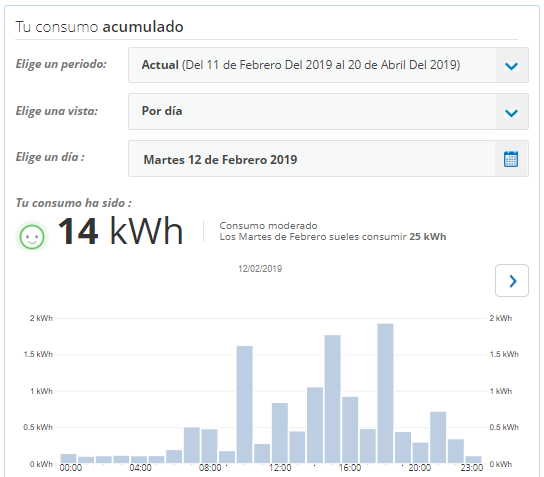
\includegraphics[width=10cm]{figs/Endesa.PNG}
    \caption{Panel de control del área cliente Endesa}
    \label{fig:endesa}
  \end{figure}
\item \textbf{Consumo interno del sistema ($ C_{int} $)}\\El sistema propuesto tiene un consumo constante de funcionamiento, cuyo valor se ha estimado en aproximadamente 2 Kw al día, alrededor de unos 0,088 watios por hora. Consta del consumo por funcionamiento de placas fotovoltaicas y realización de carga y descarga de batería.
	\item \textbf{Carga de batería (CB)}\\Cantidad de energía que se almacena en la batería para su posterior uso (almacenaje en batería). Esta variable cobra sentido en el caso de un abaratamiento de alguna fuente de generación de energía, lo que propicia que se obtenga más de la necesitada y se almacene para cuando el precio sea mayor.
	\item \textbf{Vertido al mercado eléctrico (CR)}\\Cantidad de energía que se vende al mercado eléctrico. Como particular, se puede disponer de una instalación fotovoltaica y verter energía a la red eléctrica, aunque es una práctica sujeta a numerosas trabas legales y dificultades en las que no se entrará en el desarrollo de este trabajo fin de grado. Esta energía se vertería al intramercado de red conocido como el mercado SPOT, aquel donde los activos que se compran o venden se entregan al precio de mercado del momento de la compra/venta.
\end{itemize}

Como se puede observar, el vertido al mercado eléctrico es un consumo que tiene un beneficio económico que ha de tenerse en cuenta. Existe una retribución por Kw vertido a la red dependiente del momento del día, ya que como se ha comentado antes, el valor de compra/venta del mercado SPOT varía. Para la obtención de estos valores se vuelve a hacer uso de la ya mencionada API e-sios, proporcionando a la función \textit{get\_incoming\_prices} el indicador del precio SPOT, presente en el fichero de constantes del proyecto. Análogo a la obtención del PVPC, se retorna un buffer con los 24 valores requeridos del precio SPOT correspondientes a las 24 horas a simular.\\

Aunque a priori parezca que el hecho de cargar las baterías no tiene una compensación económica, esto no es del todo correcto. Existe un beneficio económico, aunque no directo, con esta práctica. Puede ser explicado como la cantidad ahorrada por almacenar esa energía y no consumirla, ya que se ha pagado por ella. Este valor puede verse como el mínimo de los precios de las fuentes de generación de energía en el momento de la carga. Veamos un breve ejemplo:\\En la hora t se ha obtenido energía fotovoltaica a un precio de 0,11 € el Kwh. Por otro lado, se ha obtenido energía de la compañía eléctrica contratada a un precio de 0,14 € el Kwh. El beneficio económico indirecto por cargar un Kw de energía en batería en esta hora t será de 0,11 €.

\subsection{Variables de control}
Los valores de las variables definidas anteriormente son los que se intentan optimizar, pero existe otro conjunto de variables conocido como las variables de control. Aunque se denotan como variables, en el caso concreto de una simulación son constantes, ya que sus valores están predefinidos para la simulación del modelo. Este conjunto está formado por los valores de los que dependen las variables de entrada y salida y en función de los que se busca una optimización, y caracterizan tanto la simulación como la situación en una hora determinada.\\
Este conjunto está formado por:
\begin{itemize}
	\item \textbf{Fecha de inicio}\\ Valor que hace referencia al inicio de la simulación. Este valor es representado mediante el módulo datetime de Python. Datetime~\cite{Dtpy} es un módulo de la librería estándar de Python que permite manipular y trabajar con fechas. Este valor será un día y una hora de ese día.
	\item \textbf{Fecha de fin}\\ Corresponde al fin de la simulación. Siempre será 24 horas a partir de la fecha de inicio. Al igual que el anterior, se representa haciendo uso de datetime.
	\item \textbf{Número de módulos fotovoltaicos}\\ El número de módulos fotovoltaicos juega un papel fundamental. A mayor número de módulos, se producirá mas energía, pero mayor deberá ser la inversión para adquirirlos.
	\item \textbf{Precio de un módulo fotovoltaico}\\ En este trabajo el tipo de módulo fotovoltaico sera el se suele usar a nivel particular, de tamaño pequeño, con una potencia nominal en condiciones ideales de 50 watios hora~\ref{fig:pv_module}. Este modulo tiene un precio por unidad de 40 €, por lo tanto este valor tendrá el mismo valor en todas las simulaciones.
          \begin{figure}[!h]
            \centering
            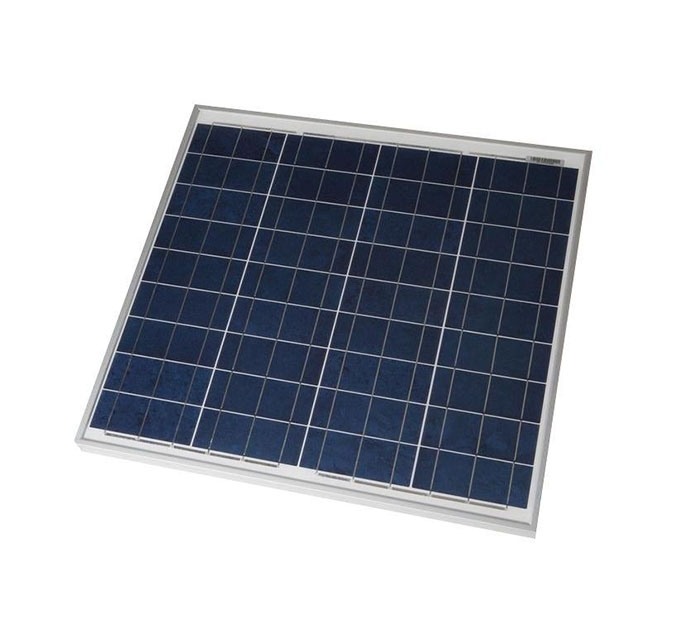
\includegraphics[width=6cm]{figs/panel_solar.jpg}
            \caption{Panel fotovoltaico de 50 W}
            \label{fig:pv_module}
          \end{figure}
	\item \textbf{Años en amortizar la inversión de los módulos fotovoltaicos}\\ El número de años en los que se desea amortizar la inversión realizada en la adquisición de los módulos fotovoltaicos, exclusivamente mediante su uso. Como se ha comentado anteriormente, no es algo trivial ya que determinará en gran medida el precio de extracción de energía fotovoltaica.
	\item \textbf{Precio de la batería}\\ En este trabajo el tipo de batería usado será una batería estacionaria~\ref{fig:bateria} compuesta por plomo abierto y gel. Este tipo de batería esta compuesta por dos vasos de 2V cada uno que disponen de un amplio rango de autonomía y una vida útil bastante larga, alrededor de unos 20 años. Son aconsejadas en instalaciones con un consumo medio (microondas, horno, lavadora, aire acondicionado, etc), es decir, perfectas para un hogar de tamaño normal. Cómo su tensión es de 2V, se debe instalar un total de 6 vasos en serie, al estar la instalación solar a 12V. Su precio es elevado debido a la gran capacidad, siendo un precio de 3900 € el de la obtención de los 6 vasos.
           \begin{figure}[!h]
            \centering
            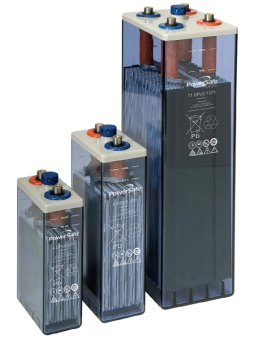
\includegraphics[width=4cm]{figs/bateria.jpg}
            \caption{Batería estacionaria}
            \label{fig:bateria}
          \end{figure}
	\item \textbf{Capacidad de la batería}\\ El tipo de batería usado, es decir, batería estacionaria de 6 vasos, tiene una capacidad total de aproximadamente 21 Kw. La profundidad de descarga de este tipo de batería es aproximadamente del 50\%, esto es, como se comento durante la explicación de las variables de entrada y salida, el tanto por ciento que se puede descargar dicha batería sin resultar perjudicial para su salud y por lo tanto afectar a su ciclo de vida útil.
	\item \textbf{Nivel de carga inicial de la batería}\\ Variable de control que define el estado inicial de la batería a la hora de realizar la simulación del modelo. Esto es la cantidad de energía que tiene almacenada la misma.
	\item \textbf{Años en amortizar la inversión de la batería}\\ Como ocurre en el caso de la inversión fotovoltaica, se debe determinar el número de años en los que se desea realizar la amortización de la inversión por adquirir la batería. Al tratarse de un valor mucho mas elevado debe ser mayor al del caso anterior, ya que si no se dispararía el precio de descargar las baterías y dejaría de ser una entrada a tener en cuenta al no resultar rentable.
\end{itemize}
Con esto quedan identificadas cada una de las variables que entran en juego en el modelo, así como su medio de adquisición.

\section{Aplicación de lógica difusa para la determinación de los estados meteorológicos}
Tal como se comentó en la iteración anterior (sección~\ref{sec:hito1}, la respuesta procesada en cada caso a la petición \textit{requests} consta de estados meteorológicos en formato de cadena de texto. Un ejemplo de respuesta del tipo texto en lenguaje natural se vió en el Listado~\ref{lst:APIresponse2}. En el Listado~\ref{lst:APIresponse1} se muestra (simplificada) la respuesta recibida en el caso de la consulta del día en curso (\textcopyright AEMET)
\begin{lstlisting}[numbers=none,float=ht,caption={Ejemplo de respuesta de la API-AEMET para el día en curso},label={lst:APIresponse1}]
{
 origen: {
	productor: "Agencia Estatal de Meteorología - AEMET. Gobierno de España",
	web: "http://www.aemet.es",
	language: "es",
	copyright: "AEMET. Autorizado el uso de la información y su reproducción citando a AEMET como autora de la misma.",
	notaLegal: "http://www.aemet.es/es/nota_legal"
 },
 elaborado: "2019-2-12",
 nombre: "Consuegra",
 provincia: "Toledo",
 prediccion: {
 	dia: [
		{
		 estadoCielo: [
					{
					 periodo: "08",
					 descripcion: "Cubierto"
					},
					{
					 periodo: "09",
					 descripcion: "Cubierto con lluvia escasa"
					},
					{
					 periodo: "10",
					 descripcion: "Cubierto con lluvia escasa"
					},
					{
					 periodo: "11",
					 descripcion: "Cubierto"
					},
					...
		 ]
		}
	}
}
\end{lstlisting}
Cómo se puede observar se diferencia de la respuesta en formato texto mostrada en el Listado~\ref{lst:APIresponse2}, pues se trata de una respuesta en formato \gls{JSON}. El lenguaje \gls{JSON} es un formato de texto simple que se utiliza para el intercambio de información y es tomado como lenguaje independiente, aunque tuvo sus inicios en Javascript, haciendo honor a su nombre (\textit{Javascript Object Notation}). En el campo 'predicción' existe un subcampo 'estadoCielo' (entre otros que se han obviado por no ser de interés en este trabajo) que contiene una lista con los estados meteorológicos de la previsión. Cada elemento de la lista contiene dos valores: período (hora del día de esa previsión) y descripción (cadena de texto que describe el estado del cielo, mismo conjunto de palabras que se emplea para encontrar las ocurrencia en el texto en el otro tipo de respuesta). Claramente existe un problema con los buffers de estados meteorológicos que se obtienen de procesar las peticiones a la \gls{API} \gls{AEMET}, ya que para la determinación de la máxima energía fotovoltaica posible en una hora t debe conocerse \gls{CMP}, la potencia nominal posible (potencia que es capaz de suministrar el módulo fotovoltaico), directamente proporcional al estado meteorológico, el cuál es un texto que describe la situación y no un valor numérico que representa los watios que puede dar un módulo en esas condiciones, y a priori no se dispone de una forma directa de relacionarlas. Por tanto, se emplea \textbf{lógica difusa} para poder resolver la problemática mencionada anteriormente.
\subsection{Lógica difusa}
La teoría de la lógica difusa proporciona un marco matemático que permite modelar la incertidumbre de los procesos cognitivos humanos para poder ser tratable por un computador. Estos procesos cognitivos hacen referencia a expresiones del tipo:
\begin{itemize}
	\item Si no vives \textit{lejos} puedes ir en bicicleta.
	\item Si hace \textit{mucho} frío llévate un chaquetón.
\end{itemize}
Los humanos son capaces de interpretar estos valores rápidamente. Sin embargo, las máquinas tienen algún que otro problema, debido a que no existe un valor cuantitativo que indique la distancia a la que se refiere la palabra \textit{lejos} o cuánto es \textit{mucho} frío. Si se intentan trasladar estas reglas a código, aparecen dificultades ya que no se puede procesar numéricamente. Una opción es definir intervalos de valores que comprenderá cada palabra (por ejemplo, tomando \textit{lejos} como la distancia comprendida entre 5 y 10 kilómetros), pero esto no es preciso ya que para un computador, la distancia de 5,01 kilómetros sería igual de lejos que 9,9 kilómetros, cuando en realidad la interpretación correcta no es así. Con esto queda a la vista que la lógica convencional no trata de forma eficiente este problema presentando numerosas limitaciones. Otro ejemplo típico es el mostrado en la Figura~\ref{fig:ejemplo_logica}, donde se puede observar como la lógica clásica interpretaría erróneamente el hecho: \textit{Una persona de dos metros es alta}, pues clasificaría una persona de 1,99 metros como no alta, mientras que la lógica difusa lo clasificaría mediante un grado de pertenencia. La solución pasa por emplear un método de razonamiento afín a la lógica difusa.\\
\begin{figure}[!h]
	\centering
	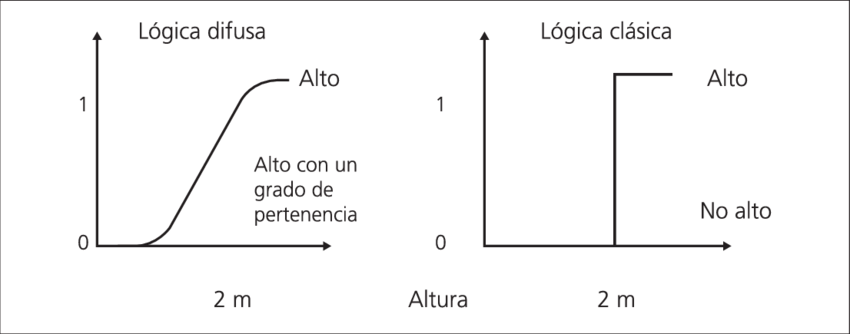
\includegraphics[width=10cm]{figs/tipos_logica.png}
	\caption{Lógica clásica vs. lógica difusa}
        \label{fig:ejemplo_logica}
\end{figure}

La lógica difusa~\cite{Morc11} permite representar matemáticamente la \textbf{incertidumbre}. Según Zadeh~\cite{Zad73}, "\textit{Cuando aumenta la complejidad, los enunciados precisos pierden su significado y los enunciados útiles pierden precisión.}", es decir, \textit{los árboles no te dejan ver el bosque}, pues prácticamente cualquier problema del mundo puede resolverse partiendo de unas variables de entrada y buscando obtener como objetivo un conjunto de variables de salida. La lógica difusa establece esta relación entre variables de forma correcta.

\subsection{Conjuntos difusos}
En la teoría de conjuntos de la lógica clásica, el grado de pertenencia puede tomar solo los valores 0 y 1, que representan que el elemento pertenece o no pertenece al conjunto. En la lógica difusa existe el concepto de \textbf{conjunto difuso}~\cite{Zad65}, establecido por Zadeh. Para trabajar con valores difusos se realiza un proceso denominado \textit{fuzzificación} que da resultados difusos. Estos resultados se someten a un proceso de \textit{defuzzificación} para transformarse en valores discretos (llamados \textit{crisp}), que tendrán un \textbf{grado de pertenecia} a los conjuntos difusos el cuál será un valor en el intervalo [0, 1], y representa cuánto pertenece al conjunto.\\

Así pues, hay un claro ejemplo de conjuntos difusos con los estados meteorológicos. En la Figura~\ref{fig:estadoCielo} la \gls{API} de \gls{AEMET}~\cite{Aemet} define los siguientes estados meteorológicos posibles (imagen obtenida de \textcopyright AEMET).
\begin{figure}[H]
	\centering
	
\includegraphics[width=17cm]{figs/estadoCieloAEMET.png}
	\caption{Posibles estados del cielo en AEMET}
	\label{fig:estadoCielo}
\end{figure}
Como se puede observar existe un gran número de estados meteorológicos posibles, y en un gran número de ellos un módulo fotovoltaico no genera energía. En estos estados el valor máximo a generar por los módulos será de 0 watios. Los estados favorables (donde un módulo genera una potencia mayor a 0 watios) serán representados como conjuntos difusos. En la Tabla~\ref{tab:estadosFavorables} se muestran cuáles son estos estados. Por ejemplo, no se puede determinar cuantos watios se producen como máximo con un tiempo \textit{Despejado} o \textit{Cubierto con nubes altas}, pero podemos mostrar los conjuntos difusos y gráficamente comprobar su distribución, para obtener un valor discreto de cada conjunto difuso, denominado el \textbf{centroide} o centro de gravedad del conjunto difuso. Este proceso es conocido como razonamiento aproximado a partir de inferencia difusa. La inferencia difusa permite obtener un valor de salida para un valor de entrada empleando la teoría de conjuntos difusos. Un ejemplo de cuestión a resolver es: \textit{¿Qué potencia pico se puede obtener de un módulo fotovoltaico si hay intervalos nubosos?}. Cómo hemos comentado anteriormente, la respuesta sería el centroide del conjunto difuso \textit{Intervalos Nubosos}. El centroide es el punto que divide el conjunto difuso en dos partes de igual masa. En la Ecuación~\ref{eq:centroide} se muestra el procedimiento para calcularlo, realizando el sumatorio de las potencias tomadas por su grado de pertenencia al conjunto dividido entre el sumatorio de dichos grados de pertenencia. En la Tabla~\ref{tab:estadosFavorables} se incluye el valor del centroide de cada conjunto difuso.\\
\begin{equation}
        \label{eq:centroide}
        Centroide = \frac{\sum_{x=i}^{n} x \mu_{A}(x)}{\sum_{x=i}^{n} \mu_{A}(x)}
\end{equation}
Para representar las variables lingüisticas, se parte del hipotético caso en el que cada variable desciende de manera ligeramente más inclinada que asciende, representando el factor de adaptación de un módulo fotovoltaico a un nuevo estado meteorológico. En la Figura~\ref{fig:fuzzySets} se pueden observar las variables lingüisticas definidas en la Tabla~\ref{tab:estadosFavorables}. En el eje horizontal se encuentra la potencia máxima posible del módulo fotovoltaico en watios y en el eje vertical el grado de pertenencia a cada variable [0,1]. Si avanzamos en el eje horizontal, vemos que el estado meteorológico es cambiante hacia estados favorables, y viceversa, ya que esto es directamente proporcional a la máxima potencia posible generada por el módulo.

Cada conjunto difuso es una función PI o \textbf{trapezoidal}, ya que no existe un único punto donde el grado de pertenencia al conjunto es 1, si no que se mantiene ese valor de pertenencia hasta que el módulo comienza a experimentar un cambio en el estado del cielo y se debe adaptar a dicho estado.

\begin{figure}[h]
	\centering
	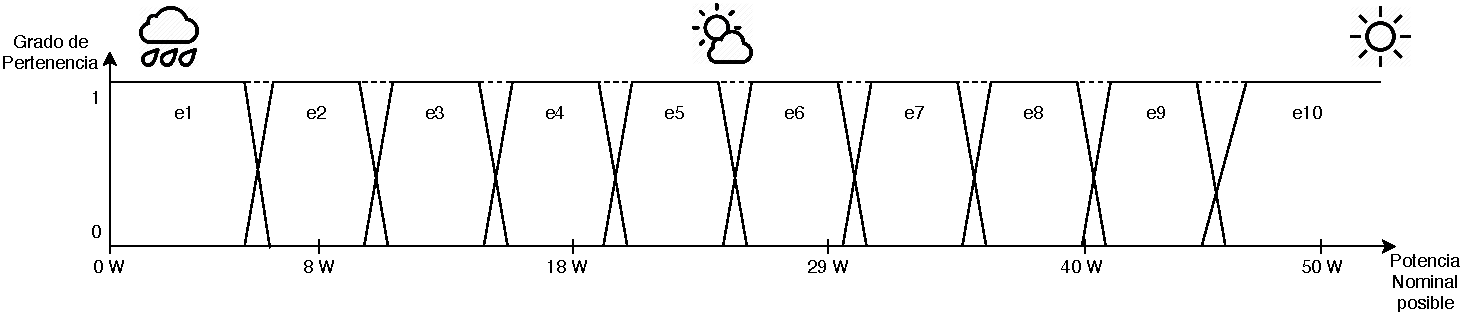
\includegraphics[width=17cm]{figs/Fuzzy_diagram.pdf}
	\caption{Conjuntos difusos de los estados meteorológicos}
        \label{fig:fuzzySets}
\end{figure}

Tal y cómo se comentó en la iteración anterior, se utilizan módulos fotovoltaicos con \gls{CMP} de 50 watios, que solo podría ser alcanzada en el estado meteorológico óptimo (\textit{Despejado}), y en función de este dato, se toman los valores para obtener los centroides.
\begin{table}[H]
        \centering
        \begin{tabular}{|c|l|c|}
                \hline
                \textbf{Etiqueta lingüistica} & \textbf{Descripción} & \textbf{Centroide} \\ \hline
                e10 & Despejado & 48 W \\ \hline
                e9 & Poco nuboso & 43.16 W \\ \hline
                e8 & Nubes altas & 38.16 W \\ \hline
                e7 & Intervalos nubosos & 33.16 W \\ \hline
                e6 & Intervalos nubosos con lluvia escasa & 28.16 W \\ \hline
                e5 & Intervalos nubosos con lluvia & 23.16 W \\ \hline
                e4 & Nuboso & 18.16 W \\ \hline
                e3 & Nuboso con lluvia escasa & 13.16 W \\ \hline
                e2 & Cubierto & 8.16 W \\ \hline
                e1 & Cubierto con lluvia escasa & 2.66 W\\ \hline
        \end{tabular}
        \caption{Variable lingüistica de la CMP}
        \label{tab:estadosFavorables}
\end{table}

El dominimo de la variable lingüistica es [0, 50] Watios. Estos valores se almacenarán en un diccionario, disponible en el fichero de constantes del proyecto (módulo \textit{project\_constants}). Dicho diccionario será usado para realizar el parseo de los estados meteorológicos obtenidos de la \gls{API} \gls{AEMET} (cadenas de texto) a valores cuantitativos (centroide del conjunto difuso), y poder ser usables por el sistema para determinar la \textbf{máxima energía fotovoltaica} que se puede obtener en un momento determinado.

\section{Creación de las relaciones y restricciones propias del modelo}
Como se comentó en el capítulo~\ref{cap:Objetivo}, la optimización se va a resolver como un \textbf{problema de satisfacción de restricciones}.\\

La programación por restricciones es una metodología software que permite resolver problemas de gran complejidad, típicamente NP. Un \gls{PSR}~\cite{Russ06} está caracterizado por:
\begin{itemize}
	\item Un conjunto de variables, donde cada variable dispone de un dominio de valores que puede tomar.
	\item Un conjunto de restricciones, que permite conocer las posibles combinaciones de las variables.
	\item La solución al PSR será la asignación de valores a las variables de forma que se satisfacen las restricciones y se alcanza el objetivo, representado típicamente como una función a optimizar.
\end{itemize}

\subsection{Variables del PSR}

El objetivo del problema es obtener valores de energía para los paneles fotovoltaicos, baterías y red eléctrica, de tal modo que se cubra la demanda energética del hogar y que el gasto económico sea el menor. Es por esto que las variables propias del problema de satisfacción de restricciones serán:
\begin{itemize}
\item \textbf{Energía fotovoltaica (EF)}. Energía obtenida de los módulos fotovoltaicos.
\item \textbf{Energía de red (ER)}. Energía importada de la red eléctrica.
\item \textbf{Energía de batería (EB)}. Energía obtenida de la batería.
\item \textbf{Consumo de batería (CB)}. Energía consumida para cargar la batería.
\item \textbf{Consumo de red (CR)}. Energía vertida a red a cambio de retribución económica.
\end{itemize}
En la Tabla~\ref{tab:domains} se muestran los dominios de estas variables.
\begin{table}[H]
        \centering
        \begin{tabular}{|c|c|}
        \hline
         \textbf{Variable del PSR} & \textbf{Dominio}\\ \hline
          Energía fotovoltaica (\gls{EF}) & $ Dom_{EF} = [0, EF_{max}] $ \\ \hline
          Energía de red (\gls{ER}) & $ Dom_{ER} = [0, +\infty) $\\ \hline
          Energía de batería (\gls{EB}) & $ Dom_{EB} = [0, +\infty) $\\ \hline
          Consumo de batería (\gls{CB}) & $ Dom_{CB} = [0, +\infty) $\\ \hline
          Consumo de red (\gls{CR}) & $ Dom_{CR} = [0, +\infty) $\\ \hline
        \end{tabular}
        \caption{Dominios de las variables del PSR}
        \label{tab:domains}
\end{table}

Las restricciones estarán definidas en función de dichas variables y cada solución al problema estará formada por un valor para cada una de estas variables. Estos valores satisfacen las restricciones y además serán los óptimos para que se produzca el menor gasto económico posible. El resto de variables (variables de control) determinarán las propias restricciones y el valor de las anteriores dependerá de éstas en una hora concreta t, entre 0 y 24h.\\

\subsection{Restricciones del PSR}
A continuación se determinan las restricciones a las que está sometido el modelo en una hora t:
\begin{itemize}
\item \textbf{Toda la energía generada debe ser consumida} (~\ref{eq:restr1}).\\ \\Hace referencia al principio básico de la energía, la energía que se produce se consume de un modo u otro, no es posible que la suma de las variables correspondientes a la generación de energía (EB, ER y EF) sea distinta a la suma de las variables que hacen referencia al consumo de energía (CR, CB, $ C_{int} $ y C). Esto debe producirse en cada una de las horas de la simulación. Así, tenemos una restricción lineal y n-aria correspondiente a la suma de las 24 horas correspondientes a una simulación, por lo que ésta restricciones a efectos prácticos es tomada como 24 restricciones a cumplir.
\begin{equation}
        \label{eq:restr1}
        \sum_{i=0}^{23} EF_{i}+ER_{i}+EB_{i} = CR_{i}+CB_{i}+C_{int}+C
\end{equation}

\item \textbf{No se puede producir energía fotovoltaica durante la noche} (~\ref{eq:restr2}).\\ \\Algo obvio, pues sin luz solar la energía fotovoltaica no es posible. Esto no está controlado en la API AEMET, ya que las peticiones relativas a la noche no reflejan una descripción propia del tiempo nocturno, si no que devuelve los mismos valores independientemente de si existe luz solar, por lo que debe manejarse mediante una restricción. Para este trabajo las horas de la noche serán las pertenecientes al intervalo temporal desde las 22:00 pm hasta las 7:00 am. Como posible trabajo futuro, podría determinarse este intervalo en función de la estación del año para que pueda ser un intervalo con mayor grado de efectividad. Se trata de una restricción unaria, donde para ciertos valores de t, EF debe ser 0. Es por esto que esta restricción a efectos prácticos es tomada como nueve restricciones (las nueve horas de noche definidas anteriormente)
\begin{equation}
        \label{eq:restr2}
        EF_{noche} = 0
\end{equation}

\item \textbf{La energía fotovoltaica generada no puede ser mayor que la máxima energía fotovoltaica en t} (~\ref{eq:restr3}).\\ \\No se puede superar el umbral de generación de energía fotovoltaica establecido por la potencia nominal máxima de esa hora t, pues se estaría violando la capacidad real de producción de los módulos fotovoltaicos del sistema. Es una restricción lineal unaria, ya que la energía fotovoltaica máxima de cada hora t es constante, pues como se comentó anteriormente, sólo es dependiente del número de módulos fotovoltaicos y la situación meteorológica (obtenida de la API AEMET). A efectos prácticos, esta restricción es tomada como 24 restricciones a cumplir referentes a las 24 horas de la simulación.
\begin{equation}
        \label{eq:restr3}
        \sum_{i=0}^{23} EF_{i} \leq EF_{i}^{max}
\end{equation}

\item \textbf{La energía obtenida de la batería no puede ser mayor que el nivel de batería actual teniendo en cuenta la profundidad máxima de descarga} (~\ref{eq:restr4}).\\ \\Básicamente no se puede obtener una cantidad de energía mayor a la posible en esa hora t, que vendrá determinada por la diferencia entre el  nivel de carga disponible al comienzo de esa hora y la capacidad máxima de la batería por la profundidad de descarga (50\%), para evitar daños en su ciclo de vida útil. Restricción unaria, pues solo involucra la variable EB, ya que el resto de elementos de la restricción son constantes en una hora t (nivel de carga actual, capacidad máxima de la batería y profundida de descarga). Al igual que las restricciones anteriores es lineal y a efectos prácticos representa 24 restricciones a cumplir.
\begin{equation}
        \label{eq:restr4}
        \sum_{i=0}^{23} EB_{i} \leq nivel_{i-1} - capacidad_{max} * profundidad_{descarga}
\end{equation}

\item \textbf{El consumo para cargar la batería no puede ser mayor que la capacidad de la misma menos el nivel restante después de t} (~\ref{eq:restr5}).\\Parecido a la restricción anterior, en esta se modela el hecho de cargar la batería (CB) en cada hora t, el cuál está condicionado por la cantidad de batería restante para completar la carga (100\%), obtenido mediante la diferencia entre la capacidad máxima de la misma y lo consumido en la hora t (nivel de carga antes de comenzar la hora t menos la energía consumida de batería en t). Restricción binaria pues involucra tanto el consumo de batería (CB) como la energía de batería (EB), siendo la capacidad máxima de la batería y el nivel de carga en t constantes. Es tomado como 24 restricciones ya que debe cumplirse en cada una de las 24 horas de una simulación.
\begin{equation}
        \label{eq:restr5}
        \sum_{i=0}^{23} CB_{i} \leq capacidad_{max}- (nivel_{i-1} - EB_{i})
\end{equation}

\end{itemize}

Por lo tanto, a efectos prácticos, el PSR tiene 81 restricciones que satisfacer para determinar los valores de las variables.

\subsection{Función Objetivo}
Cómo se ha comentado antes, un problema de satisfacción de restricciones está determinado por un conjunto de variables y sus dominios, un conjunto de restricciones sobre esas variables y un objetivo. Por el momento se dispone de los dos primeros, por lo que en este apartado se procede a determinar el último, \textbf{la función objetivo}.\\

Un PSR que cuenta únicamente con variables y restricciones para esas variables podrá tener numerosas soluciones, representadas como una tupla con valores para cada variable. Añadiendo un objetivo al PSR se consigue unificar la solución, pues de todas esas soluciones, sólo una optimizará un objetivo concreto, y contendrá los valores óptimos de cada variable para ello.\\

Como se ha comentado a lo largo del desarrollo de este \gls{TFG}, el objetivo del problema es \textbf{minimizar el gasto económico} producido mediante la optimización de energía en cada simulación de 24 horas, por lo tanto se buscarán valores de las variables que, además de satisfacer el conjunto de restricciones, sean óptimos para que el gasto económico sea mínimo. Éste gasto económico es dependiente del precio en la hora t de cada una de las energías que representan las variables. De estos precios se habló y se implementó la forma de obtenerlos en la Iteración~\ref{sec:hito1}. Sus valores son constantes en cada hora t. Dicho esto, la función objetivo a minimizar está formada por el sumatorio de los costos económicos en cada hora t, por lo que representa el gasto económico de toda la simulación (~\ref{eq:funcionObjetivo}).
\begin{equation}
\label{eq:funcionObjetivo}
f(x) = \sum_{i=0}^{23} EF_{i}P_{i}^{F} + ER_{i}P_{i}^{R_{PVPC}} + EB_{i}P_{i}^{B_{out}} - CB_{i}P_{i}^{B_{in}} - CR_{i}P_{i}^{R_{SPOT}}
\end{equation}
Siendo:
\begin{itemize}
\item $ EF_{i}P_{i}^{F} $: Gasto económico producido al generar energía fotovoltaica en la hora t.
\item $ ER_{i}P_{i}^{R_{PVPC}} $: Gasto económico producido al importar energía a la compañía eléctrica en la hora t.
\item $ EB_{i}P_{i}^{B_{out}} $: Gasto económico producido al descargar la batería en la hora t.
\item $ CB_{i}P_{i}^{B_{in}} $: Ganancia económica producida al cargar la batería en la hora t.
\item $ CR_{i}P_{i}^{R_{SPOT}} $: Ganancia económica producida al verter energía al mercado eléctrico en la hora t.
\end{itemize}

En cada simulación se buscará que el valor de $ f(x) $ sea el menor posible y la solución al PSR de esa simulación son los valores que deben tomar las variables para hacerlo posible.

\subsection{Implementación de la clase Simulation}
Vistos los apartados anteriores, es la hora de implementar una clase para representar el modelo de simulación y poder crear objetos que representan una simulación concreta. Esta clase se llama \textbf{Simulation} (Figura~\ref{fig:simulation} y está disponible en el módulo simulation. Los atributos de la clase Simulation serán las variables de control que tendrá cada objeto correspondiente a una simulación:
\begin{itemize}
        \item start: variable de control relativa a la fecha de inicio de la simulación. Es de tipo datetime.
        \item end: variable de control relativa a la fecha de fin de la simulación. Al igual que start, es una variable de formato fecha (datetime).
        \item ef\_price: variable de control referente al precio de generar energía fotovoltaica. Se trata de un número tipo float, pues tendrá el mismo valor en toda la simulación (se obtiene a partir de la inversión realizada).
        \item er\_price: variable de control referente a los precios que tendrá el \gls{PVPC} en cada hora de la simulación. Es una lista de 24 elementos de tipo float.
        \item eb\_price: variable de control referente al precio de descargar la batería. Es un número de tipo float ya que será igual en las 24 horas de la simulación.
        \item cr\_price: variable de control referente a los precios SPOT en cada hora de la simulación, es decir, el precio del vertido de energía a la red eléctrica.
        \item cb\_price: variable de control referente a los precios de cargar la batería. Como es dependiente de los precios de energía fotovoltaica y de red de cada hora t, se trata de una lista con 24 valores.
        \item battery\_capacity: variable de control referente a la capacidad total de la batería. Variable de tipo float.
        \item battery\_level: variable de control que representa el nivel inicial de carga de la batería. Variable de tipo float.
        \item discharge\_depth: variable de control referente a la profundidad de descarga permitida en la batería. Variable de tipo float.
        \item max\_ef\_buffer: Más que una variable de control, representa los 24 valores máximos posibles de energía fotovoltaica, obtenidos como se comentó anteriormente mediante la información de la API AEMET y el número de módulos fotovoltaicos, por tanto, se trata de una lista de 24 valores.
        \item c\_int: referente a la variable de control del consumo interno del sistema. Variable de tipo float.
        \item c: referente al consumo del hogar, lista de los 24 valores con el consumo del hogar en las 24 horas de la simulación.

Las funciones de esta clase sirven para calcular algunos de los atributos anteriores. En la Figura~\ref{fig:simulation} se muestra la clase UML de Simulation.
\end{itemize}

\begin{figure}[H]
        \centering
        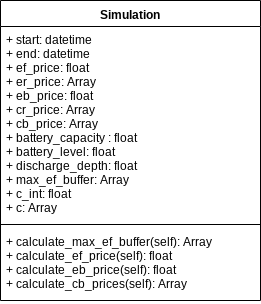
\includegraphics[width=6cm]{figs/simulation_class.png}
        \caption{Clase Simulation}
        \label{fig:simulation}
\end{figure}

En la próxima iteración se implementará cada una de las restricciones para ejecutar la simulación.

\section{Generación optimizada de energía mediante programación lineal}
Cómo se comentó anteriormente, éste PSR dispone de 81 restricciones. Además, no interesa cualquiera de las soluciones posibles si no que debe buscarse la solución más óptima de todas. Por lo tanto para su resolución deberá emplearme algún procedimiento lo suficientemente potente para contemplar ambos requisitos.
\subsection{Programación Lineal}
La programación lineal~\cite{Loom64} tiene como objetivo optimizar una función lineal cuyas variables están sujetas a un conjunto de restricciones lineales.
Se trata de un campo de la matemática muy efectivo para la resolución de problemas donde se desea sacar el mayor provecho de una situación.\\

Históricamente, el concepto de programación lineal debe su nombre a John Von Neumann (1947), uno de los matemáticos más importantes del siglo XX gracias a sus contribuciones en las ciencias de la computación; y a George Dantzig (1947), cuyo trabajo intentaba asignar 70 puestos de trabajo a 70 personas mediante programación lineal. Las permutaciones necesarias para la asignación óptima de dichos puestos era factorial de 70 (70!), algo enorme, pues el número de combinaciones de variables es inmenso. Curiosamente, mediante programación lineal el problema se resuelve en un momento pues el número de combinaciones se reduce en su mayor parte. La programación lineal puede ser aplicable a numerosos problemas comunes tales como:
\begin{itemize}
\item Asignación de horarios a profesores en un centro educativo para obtener la mayor productividad a la par que comodidad para profesor y alumno.
\item Distribución de elementos en almacenes de tal modo que se reduzca el costo de almacenamiento teniendo en cuenta la limitada capacidad.
\item Distribución de bienes entre compradores y consumidores de tal modo que las ganancias del intermediario sean máximas.
\end{itemize}
Cómo se puede observar, el problema de este trabajo fin de grado está muy relacionado con el último ejemplo, pues se distribuye cantidad de energía entre fuentes de entrada y fuentes de salida de manera óptima para garantizar un gasto mínimo de consumo energético.\\

Para un problema de programación lineal pueden existir varios casos en su resolución:
\begin{itemize}
\item Existe una solución óptima.
\item Existen varias soluciones óptimas.
\item No existe solución.
\item Existen soluciones infinitas.
\end{itemize}
La situación deseada es la primera, pero puede ocurrir alguno de los otro casos. Estas situaciones pueden resolverse convirtiendo las restricciones que son inecuaciones (desigualdades) en igualdades.\\

Existen varios métodos de programación lineal. El más utilizado es conocido como el \textbf{método Simplex}, pues es muy potente debido a que se basa en evaluar solo algunos puntos extremos mediante dos condiciones:
\begin{itemize}
\item \textbf{Optimalidad}. La solución inferior relativa al punto de solución actual no se tiene en cuenta.
  \item \textbf{Factibilidad}. Una vez se encuentra una solución básica factible, sólo apareceran soluciones factibles.
\end{itemize}
Otro método de programación lineal es el método de ramificación y acotamiento \textit{branch and bound}, el cuál divide el problema en varios subproblemas de programación lineal, acotamiento que permite obtener soluciones óptimas que se mejorar por cada subproblema.\\

En el ámbito de las ciencias de la computación existen librerías que permiten emplear algoritmos de programación lineal para la resolución de problemas de optimización. En este trabajo fin de grado se empleará \textbf{SciPy}, un ecosistema de librerías de código abierto con numerosas herramientas para matemáticas, ciencia e ingeniería.

\subsection{Optimización con SciPy}
Scipy~\cite{Scip} proporciona un conjunto de paquetes de computación científica para el lenguaje Python como son Numpy, Scipy, Matplotlib, iPython, SymPy y Pandas. En este caso el trabajo se centra en el módulo Scipy.optimize~\cite{SciOp}, que contiene las herramientas de Scipy para optimización. Proporciona numerosos algoritmos de optimización para uso común:
\begin{itemize}
\item Minimización sin restricciones y restringida de funciones escalares multivariadas.
\item Optimización global mediante fuerza bruta.
\item Minimización de mínimos cuadrados.
\item Minimización de funciones univariantes escalares y búsqueda de soluciones.
\item Solución de sistemas de ecuaciones multivariables con una gran cantidad de algoritmos.
\end{itemize}
Para el caso propio de este trabajo fin de grado en que se el objetivo es minimizar una función sujeta a un gran conjuntos de restricciones, lo más conveniente es hacer uso del módulo \textbf{linprog} de Scipy.optimize, específico para trabajar con programación lineal. Resuelve problemas del tipo definido en el listado~\ref{lst:linprog}, donde:
\begin{itemize}
\item A\_ub representa los coeficientes de las restricciones definidas como inecuaciones.
\item b\_ub representa las constantes del tipo de restricción inecuación.
\item A\_eq representa los coeficientes de las restricciones de igualdad, es decir, ecuaciones.
\item b\_eq representa las constantes del tipo de restricción de igualdad.
\item (lb, ub) representan los límites inferior y superior del dominio de la variable x.
\item c es la función a minimizar, dependiente de la variable x.
\end{itemize}
\begin{lstlisting}[language=Python,float=ht,numbers=none,caption={Tipo de problema aplicable a Scipy.optimize.linprog},label={lst:linprog}]
  # Minimizar:
  c @ x
  # Sujeto a:
  A_ub @ x <= b_ub
  A_eq @ x == b_eq
  lb <= x <= ub
\end{lstlisting}
El caso particular de este trabajo se adapta perfectamente a dicho modelo de problema. Pero antes de implementar el algoritmo linprog, se deben implementar cada una de las restricciones del modelo, algo complejo en este caso pues existen numerosas restricciones al tratarse de una función lineal, pues cada una de las variables involucradas en la función a minimizar~\ref{eq:funcionObjetivo} tendrá realmente 24 valores, correspondientes a las 24 horas de la simulación, y desde el punto de vista de la implementación, será tenido en cuenta como 24 variables distintas.\\

Antes de implementar cada una de las restricciones, se debe hacer una modificación en la clase Simulation. Se añaden cinco nuevos atributos a la clase:
\begin{itemize}
\item \textbf{f}: Esta variable representa la función objetivo (véase la ecuación~\ref{eq:funcionObjetivo}), expresada como una lista con los coeficientes de cada variable en la función los cuáles representan el precio del tipo de energía asociado a la variable. Al tratarse de un sumatorio de 24 iteraciones y contener 5 variables en la expresión, esta lista contendrá 120 elementos resultantes de la suma entre los 24 valores de cada una de las variables. Para dotar de valores a la lista se ha implementado la función \textit{generate\_function\_coeficients()}, que mediante 24 iteraciones concatena a la lista el valor correspondiente de cada coeficiente de variable, que se encuentran en los atributos de clase definidos en la iteración 3 (Véase la representación UML de Simulation en la figura~\ref{fig:simulation}). Esta variable se corresponde con \textit{c} en el modelo de problema para Scipy Linprog del listado~\ref{lst:linprog}.
\item \textbf{A\_ub, b\_ub}: Cómo se comentó anteriormente representan las restricciones del tipo inecuación. En A\_ub se almacenan en una lista los coeficientes de las inecuaciones en una lista por restricción, de tal modo que se tiene una lista de listas (lista de dos dimensiones) del tipo: [[coeficientes restr. 1], [coeficientes restr.2], ...]. En b\_ub se tiene una lista con las constantes de las inecuaciones, por lo que el tamaño de b\_ub y A\_ub debe ser igual para que se realice el \textit{matching} de coeficientes con constantes por inecuación.
\item \textbf{A\_eq, b\_eq}: Similar a las dos listas anteriores, pero en este caso se trata de las restricciones de igualdad. Las lista tienen el mismo formato.
\end{itemize}
Éstas variables serán primordiales a la hora de ejecutar el algoritmo linprog pues de sus valores serán dependientes los resultados para cada variable. Definidas las variables que contendrán los valores de las restricciones se pasa a la implementación de dichas restricciones.
\subsection{Implementación de las restricciones del tipo 1}
La restricción 1 se corresponde con que toda la energía generada debe ser consumida (Véase la ecuación~\ref{eq:restr1}). Se trata de una restricción de igualdad, por lo que deben dotarse de valor A\_eq y b\_eq. Es una restricción lineal por lo que desde el punto de vista de la implementación se traduce en 24 restricciones, una por hora de la simulación. En el listado~\ref{lst:restr1} se muestra la función \textit{generate\_restriction\_1()} que realiza dicha tarea.\\
\begin{lstlisting}[language=Python,float=ht,caption={Restricciones del tipo 1},label={lst:restr1}]
def generate_restriction_1(self):
    for i in range(0, 24):
        restr_coef = [0]*5*24
        restr_coef[i*5] = 1
        restr_coef[i*5+1] = 1
        restr_coef[i*5+2] = 1
        restr_coef[i*5+3] = -1
        restr_coef[i*5+4] = -1
        self.A_eq.append(restr_coef)
        self.b_eq.append(self.c_int + self.c[i])
\end{lstlisting}

Primero se deben mostrar a la izquierda de la restricción las variables y a la derecha las constantes. En A\_eq se debe concatenar una lista por restricción del sumatorio que contendrá los valores 0 o 1 en función de la condición mostrada en el listado~\ref{lst:coef}
\begin{lstlisting}[numbers=none,float=ht,caption={Condición para dotar de valor los coeficientes},label={lst:coef}]
  Si la variable de esa posición aparece en la restricción
      restr_coef[posicion] = 1
  Si no
      restr_coef[posicion] = 0
\end{lstlisting}
Cómo se puede observar en el listado~\ref{lst:restr1}, por cada iteración de las 24 (correspondientes a las 24 horas de la simulación) primero se crea una lista \textbf{restr\_coef} con solo valores 0. Ésta lista dispone de 120 elementos, pues la restricción es realmente el sumatorio de 24 restricciones y existen 5 variables en la expresión (EF, ER, EB, CR y CB). Cómo resultado se obtendrá en A\_eq 24 listas de 120 elementos cada una, de los cuáles todos toman el valor 0 excepto los relativos a las posiciones de las variables que entran en juego en la restricción de esa iteración. Es primordial que se preserve el orden de ordenamiento de las variables en todas las restricciones. Deben tener el mismo orden que en la función objetivo y tomar 1 si aparecen o 0 si no (Podrán tomar el valor -1 si van precedidas de una resta en la restricción). En el caso de b\_eq, se concatenan 24 valores, uno por iteración, correspondientes l valor constante de la restricción de esa iteración.\\Obsérvese cómo se realizaría la primera iteración, correspondiente a la hora 0 de la simulación:\\

\textit{Deben dotarse con 1 $ EF_{0} $, $ ER_{0} $ y $ EB_{0} $, pues su coeficiente en la restricción es +1. Deben dotarse con -1 $ CR_{0} $ y $ CB_{0} $, pues su coeficiente es -1 en la restricción. El resto de elementos de la lista deben ser 0 (Correspondientes al resto de coeficientes de variables para i=1,2,3..). Ésta lista se concatena en A\_eq. En b\_eq se concatena el valor constante de esta restricción, que es $ c_{int} + C_{i}^{prop} $. Con esta queda implementada la restricción de tipo 1 correspondiente a la hora 0 de la simulación.}

\subsection{Implementación de las restricciones del tipo 2}
La restricción 2 hace referencia a que no se puede producir energía fotovoltaica durante la noche (Véase la ecuación~\ref{eq:restr2}). En este trabajo fin de grado se definen estos valores como los comprendidos entre las 9:30 pm y las 7:00 am. Como se observa en el listado~\ref{lst:restr2}, para generar las restricciones de este tipo, en cada iteración se inicializa la lista de 120 valores con ceros de manera análoga a las restricciones de tipo 1. Después, para determinar la hora real correspondiente de la iteración en curso, se debe sumar a la hora de inicio de la simulación el número de iteración actual. El uso del módulo de la librería estándar de Python \textit{datetime}~\cite{Dtpy} hace que sea posible manejar variables en formato hora o fecha. En las iteraciones en las que la hora actual esté comprendida en las definidas cómo horas nocturnas, el valor de la posición de EF (energía fotovoltaica) en esa iteración tomará el valor 1. Éstas listas resultantes de cada iteración se van concatenando con A\_eq, pues son restricciones de igualdad. En cuanto a b\_eq, por cada iteración se concatena un 0, pues el valor constante de esta restricción es 0 debido a que la energía fotovoltaica de noche es nula. Tras la ejecución de la función \textit{generate\_restriction\_2()} A\_eq cuenta con 24 listas mas, que son las 24 restricciones del tipo 2.
\begin{lstlisting}[language=Python,float=ht,caption={Restricciones del tipo 2},label={lst:restr2}]
def generate_restriction_2(self):
    for i in range(0, 24):
        restr_coef = [0]*5*24
        time = (self.start+dt.timedelta(hours=i)).time()
        if time >= dt.time(21, 30) or time <= dt.time(7, 00):
            restr_coef[i*5] = 1
        self.A_eq.append(restr_coef)
        self.b_eq.append(0)
\end{lstlisting}
\subsection{Implementación de las restricciones del tipo 3}
Las restricciones del tipo 3 hacen que se cumpla que la energía fotovoltaica generada no puede ser mayor que la máxima energía fotovoltaica en t, siendo t cada hora de la simulación (Véase la ecuación~\ref{eq:restr3}). Se trata de una restricción de tipo inecuación, por lo que en este caso deberán concatenarse sus valores a A\_ub y b\_ub. En la variable de clase \textit{self.max\_ef\_buffer} se dispone de una lista con los 24 valores correspondientes a la energía fotovoltaica máxima de cada hora de la simulación. Cada elemento de esta lista representa la parte constante de cada restricción de este tipo, por ello, en cuanto a b\_ub se refiere, basta con concatenar \textit{self.max\_ef\_buffer}. En el caso de la parte de variables (A\_ub), al igual que en los casos anteriores se realizan 24 iteraciones correspondientes a las 24 horas de la simulación, y en cada una de ellas, la lista de 120 elementos toma el valor 1 únicamente en la posición relativa a la energía fotovoltaica, pues es la única que entra en juego en este tipo de restricción.La lista generada en cada iteración se concatena con el resto de restricciones en A\_ub.
\begin{lstlisting}[language=Python,float=ht,caption={Restricciones del tipo 3},label={lst:restr3}]
def generate_restriction_3(self):
    for i in range(0, 24):
        restr_coef = [0]*5*24
        restr_coef[i*5] = 1
        self.A_ub.append(restr_coef)
    self.b_ub.extend(self.max_ef_buffer)
\end{lstlisting}
\subsection{Implementación de las restricciones del tipo 4}
Las restricciones de tipo 4 hacen que se cumpla que la energía obtenida de la batería no puede ser mayor que el nivel de batería actual teniendo en cuenta la profundidad máxima de descarga (Véase la ecuación~\ref{eq:restr4}). Son restricciones de tipo inecuación por lo que deben modificarse A\_ub y b\_ub. En este caso, la restricción correspondiente a la hora 0 de la simulación debe separarse de las restantes, pues en ese punto la cantidad de carga de la batería se obtiene directamente de la variable de clase que contiene el nivel inicial de batería (\textit{self.battery\_level})~\ref{eq:restr4t1} y en el resto de casos se obtiene mediante un conjunto de operaciones~\ref{eq:restr4t2}. Esto permite calcular el nivel actual de batería en la hora i a partir de la que hubo inicialmente, mediante el sumatorio de las cargas y descargas que se han realizado desde que comenzó la simulación. En el listado~\ref{lst:restr4} se puede observar la función \textit{generate\_restriction\_4()}, encargada de la implementación de las restricciones de tipo 4 comprendidas entre las horas 1 y 24 de la simulación. Por cada iteración, en la lista de coeficientes se coloca un uno en la posición relativa a EB, pues es la dependiente de esta restricción. Después, se realizan iteraciones desde 0 hasta la iteración anterior a la actual, para comprobar el nivel actual de batería, posicionando los valores 1 en EB y -1 en CB. Cuando la lista de coeficientes está completa en esa iteración, se añade a A\_ub, y en b\_ub se concatena la parte constante de este tipo de restricción, que viene a ser la diferencia entre el nivel inicial de batería y la capacidad de la misma por su profundidad de descarga.
\begin{equation}
  \label{eq:restr4t1}
  EB_{0} \leq initial\_level - capacity * depth
\end{equation}
\begin{equation}
  \label{eq:restr4t2}
  EB_{i} \leq initial\_level + \sum_{t=0}^{i-1}(-EB_{t}+CB_{t}) - capacity * depth
\end{equation}
\begin{lstlisting}[language=Python,float=ht,caption={Restricciones del tipo 4},label={lst:restr4}]
def generate_restriction_4(self):
    for i in range(1, 24):
        restr_coef = [0]*5*24
        restr_coef[i*5+2] = 1
        for j in range(0, i-1):
            restr_coef[j*5+2] = 1
            restr_coef[j*5+4] = -1
        self.A_ub.append(restr_coef)
        self.b_ub.append(self.battery_level
            -self.battery_capacity*self.discharge_depth)
\end{lstlisting}
\subsection{Implementación de las restricciones del tipo 5}
Las restricciones de tipo 5 se encargan de que el consumo para cargar la batería no pueda ser mayor que la capacidad de la misma menos el nivel restante después de t (Véase la ecuación~\ref{eq:restr5}). Las restricciones de este tipo son muy parecidas a las de tipo 4, con la diferencia de que las retricciones de tipo 4 se encargan de regular la energía que se descarga de la batería y las restricciones de tipo 5 regulan la energía que se carga a la batería. La hora 0 de la simulación debe implementarse aparte análogamente al tipo anterior, pues el nivel actual de batería se determina en función de las cargas y descargas que se han producido desde que comenzó la simulación. En este caso la restricción de la hora 0 es muy sencilla pues tras agrupar a la izquieda de la inecuación las variables y a la derecha las constantes y ordenar las variables preservando el orden de \textit{f} se obtiene la restricción~\ref{eq:restr5t1}. Para implementar esta restricción simplemente se debe dar valor de -1 a la posición relativa a $ EB_{0} $ y 1 a la posición relativa a $ CB_{0} $, para después añadir a sus respectivas listas la lista de coeficientes y el valor constante de la restricción. Para el resto de restricciones de este tipo (hora 1 a 24) se usa la función \textit{generate\_restriccion\_5()} cuya traza es similar a \textit{generate\_restriccion\_4()} exceptuando los valores que toman las posiciones relativas a las variables dependientes de la restricción.
\begin{equation}
  \label{eq:restr5t1}
  CB0 - EB0 <= capacity - initial_level
  -EB_{0} + CB_{0} \leq capacity - initial\_level
\end{equation}
\begin{lstlisting}[language=Python,float=ht,caption={Restricciones del tipo 5},label={lst:restr5}]
def generate_restriction_5(self):
    for i in range(1, 24):
        restr_coef = [0]*5*24
        restr_coef[i*5+4] = 1
        restr_coef[i*5+2] = -1
        for j in range(0, i-1):
            restr_coef[j*5+2] = -1
            restr_coef[j*5+4] = 1
        self.A_ub.append(restr_coef)
        self.b_ub.append(self.battery_capacity - self.battery_level)
\end{lstlisting}
\subsection{Generación optimizada de energía}
Una vez implementadas todas las restricciones necesarias del PSR es la hora de implementar el algoritmo linprog de Scipy. El método \textit{optimize()} de la clase Simulation se encarga de esta tarea. En ella deben llamarse todos los métodos encargados de las restricciones, para así poder contener en A\_eq, b\_eq, A\_ub y b\_ub los datos de variables y constantes necesarios. Después deben determinarse los límites que pueden tomar las variables, definidos en la iteración anterior. Finalmente se efectúa el algoritmo linprog sobre todos los datos y se obtiene como respuesta un conjunto de valores que han de ser interpretados, para lo que se añaden a la clase Simulation las siguientes funciones auxiliares:
\begin{itemize}
\item \textbf{store\_result(result)}: Se encarga de almacenar en un fichero los resultados obtenidos, indicando fecha de simulación, gasto económico producido y cantidad de energía de cada fuente de entrada y salida por horas. Esta información es almacenada en un fichero llamado \textit{simulation\_fecha.txt}, que sirve como reporte de la simulación. Para obtener cada valor se itera sobre la lista de valores en bruto \textbf{\textit{res.x.to\_list()}} separando cada valor de variable en su iteración y variable correspondiente.
\item \textbf{prepare\_result(result)}: Se encarga de procesar una salida a la simulación alternativa a la anterior, pues retorna los resultados utilizando el formato json. Ésto será útil cuando se haga una petición de simulación desde el servidor y deba devolverse el resultado en este formato para poder ser procesado fácilmente. Se utiliza el método \textit{json.dumps()} para generar el objeto json a partir de un diccionario clave-valor (Véase el listado~\ref{lst:resultJson}). La función \textit{self.prepare\_hours(values)} procesa la lista de valores de variables en bruto a un diccionario clave-valor.
\begin{lstlisting}[language=Python,float=ht,caption={Función de procesamiento del resultado a formato json},label={lst:resultJson}]
def prepare_result(self, res):
    values = res.x.tolist()
    data = {
      "start" : self.start.strftime("%Y-%m-%d %H:%M:%S"),
      "end" : self.end.strftime("%Y-%m-%d %H:%M:%S"),
      "result" : res.fun,
      "hours" : self.prepare_hours(values)
    }

    return json.dumps(data)
\end{lstlisting}
\end{itemize}
Puesto que ya se cuenta con el esqueleto del proceso para llevar a cabo una simulación, se procede a realizar un caso de prueba del lunes 11 de Marzo de 2019.
\subsection{Caso de prueba: Simulación del 11 de Marzo}
Tal y cómo se explicó en la primera iteración, en el Área Cliente de Endesa es posible obtener el consumo realizado por horas de un día determinado. Esto va a permitir conocer cuál fue el consumo del 11 de Marzo y, gracias al trabajo realizado con la API e-sios~\cite{Ree}, poder saber cuál fue la cuantía económica que supuso el consumo total de ese día, para así poder comparar con el gasto económico que se obtendrá de la simulación.\\

El 11 de marzo en el hogar del alumno se produjo un consumo total de 7 KWh. El precio voluntario al pequeño consumor (PVPC) por defecto de ese día obtuvo cómo valor medio 0.12 euros, por lo tanto cómo mínimo el consumo del día supuso un gasto de 0.84 euros. El fichero de texto que contiene el consumo diario de Endesa sigue el formato mostrado en el listado~\ref{lst:11marzo} (\textcopyright Endesa S.A.)\\

\begin{lstlisting}[float=ht,numbers=none,caption={Fichero de consumo por horas de Endesa},label={lst:11marzo}]
CUPS:				ESXXXXXXXXXXXXXXXXXXXX
Fecha :				11/03/2019
Fecha y hora de extracción :	23/03/2019 10:57:52
Tarifa :			No se encontró la tarifa
  Fecha 			   Hora 			    Consumo (Wh)
2019-03-11			00:00-01:00				110.0
2019-03-11			01:00-02:00				80.0
2019-03-11			02:00-03:00				166.0
2019-03-11			03:00-04:00				141.0
2019-03-11			04:00-05:00				95.0
2019-03-11			05:00-06:00				126.0
2019-03-11			06:00-07:00				186.0
2019-03-11			07:00-08:00				217.0
2019-03-11			08:00-09:00				568.0
2019-03-11			09:00-10:00				692.0
2019-03-11			10:00-11:00				280.0
2019-03-11			11:00-12:00				216.0
2019-03-11			12:00-13:00				149.0
2019-03-11			13:00-14:00				348.0
2019-03-11			14:00-15:00				677.0
2019-03-11			15:00-16:00				339.0
2019-03-11			16:00-17:00				368.0
2019-03-11			17:00-18:00				192.0
2019-03-11			18:00-19:00				202.0
2019-03-11			19:00-20:00				175.0
2019-03-11			20:00-21:00				648.0
2019-03-11			21:00-22:00				479.0
2019-03-11			22:00-23:00				318.0
2019-03-11			23:00-00:00				270.0

Total (Wh):				7042.0
\end{lstlisting}
Mediante la función \textit{read\_from\_file()} del módulo \textit{client\_consumption} se procesa el fichero de consumo, se establecen los consumos en la unidad de KWh y se retorna una lista con los 24 consumos de las 24 del día, en este caso 11 de marzo. Esta lista será el valor que toma la variable de Simulation \textit{self.c}. Debido a que aún no se dispone de interfaz ni servidor, para ejecutar la simulación se ha empleado el intérprete de comandos ipython3. Se debe crear un objeto simulación con los argumentos necesarios explicados a lo largo de este capítulo y que se pueden observar en la clase UML de Simulation (Figura~\ref{fig:simulation}). Tras instanciar en un objeto la simulación, se debe invocar el método \textit{optimize()} que implementa las restricciones y ejecuta el algoritmo de programación lineal, obteniendo como salida el contenido del listado~\ref{lst:output}.\\

\begin{lstlisting}[language=bash,float=ht,numbers=none,caption={Salida del algoritmo \textit{linprog}},label={lst:output}]
fun: 0.6187091110614097
message: 'Optimization terminated successfully.'
nit: 236
slack: array([ 8.16000000e-01,  8.16000000e-01,  8.16000000e-01,
        8.16000000e-01,  2.66000000e-01,  2.66000000e-01,
        2.66000000e-01,  2.66000000e-01,  0.00000000e+00,
                                      . . .
        5.91880000e+00,  4.68600000e+00,  1.05000000e+01,
        5.02480000e+00,  1.05000000e+01,  1.05000000e+01])
status: 0
success: True
x: array([0.00000000e+00, 1.98800000e-01, 0.00000000e+00,
       0.00000000e+00, 0.00000000e+00, 0.00000000e+00,
       1.68800000e-01, 0.00000000e+00, 0.00000000e+00,
                                     . . .
       0.00000000e+00, 0.00000000e+00, 0.00000000e+00,
       3.58800000e-01, 0.00000000e+00, 0.00000000e+00])
\end{lstlisting}
Esta información es difícil de interpretar estando fuera de contexto.
\begin{itemize}
\item \textit{fun} es el resultado que toma la función \textit{f(x)} (Función~\ref{eq:funcionObjetivo}) como resultado de asignar a las variables los valores de la optimización. Dicho valor representa el \textbf{gasto económico} producido para el día simulado. Cómo se puede observar, se trata de 0.61 euros frente a los 0.84 euros que supuso el consumo del día utilizando solamente la energía de la compañia eléctrica. Se ha producido un ahorro del 27.38\% lo cuál es bastante significativo, teniendo en cuenta que el valor medio del PVPC del día 11 de marzo fue relativamente bajo con respecto al valor que suele oscilar (0.15 euros).
\item \textit{message} devuelve \textit{feedback} sobre si la optimización ha tenido o no éxito, tomando en los campos \textit{status} y \textit{success} los valores 0 y True en caso de éxito; y los valores 1 y False en caso de error.
\item \textit{nit} hace referencia a las iteraciones realizadas sobre las variables para determinar el valor óptimo obtenido. En este caso se han realizado 236 iteraciones.
\item \textit{slack} contiene un array con los valores de las variables de holgura, donde cada variable de holgura corresponde con una de las restricciones de desigualdad.
\item \textit{x} contiene el array en bruto de valores de variables que han hecho posible la optimización. Esta información ha de ser tratada y clasificada para poder ser interpretada, por lo que mediante la función \textit{store\_result()} se ha generado un fichero de reporte de simulación que contiene el valor de cada variable (EF, ER, EB, CB, CR, C y $ C_{int} $) en cada una de las horas de la simulación. Estos valores representan la cantidad de energía en KWh que debe tomarse en cada variable para producir la minimización del gasto económico.
\end{itemize}
Véase el Anexo A pues contiene el listado~\ref{lst:simulationReport} con la información procesada de la simulación.\\Cómo se puede observar, en la hora de comienzo de la simulación (0:00), la única fuente de energía es la energía de red, pues una de las restricciones implementadas es que durante la noche la energía fotovoltaica no es posible, y la batería aún no se ha cargado para permitir su extracción. Se puede observar que en algunas horas se genera más energía de la necesaria para satisfacer el consumo (C + $ C_{int} $). Esto es debido a que mediante la API aemet~\cite{Ree} se comprueba que en ese momento el precio PVPC se encuentra relativamente bajo por lo que resulta rentable importar más energía de la necesaria y almacenarla en batería para una hora en la que los precios suban. Es el caso de lo ocurrido en la hora 2:00 a.m. por ejemplo. A partir del amacener comienza a tenerse en cuenta la energía fotovoltaica, es el caso de la hora 8:00 a.m., donde se aprovecha su potencial para importar mucha más energía de la requerida y se almacena (Se requieren 0.65 KWh pero sin embargo son generados 0.816 KWh, aprovechando la diferencia para cargar la batería). Esto permite que en horas donde por causas meteorológicas (API AEMET~\cite{Aemet}) no sea posible emplear energía fotovoltaica se tengan alternativas a la energía de red, o también durante la noche, como es el caso de la hora 11:00 p.m., cuando la energía fotovoltaica no es posible y la energía de red tiene un precio más alto, se obtenga la totalidad de la energía requerida de la batería (EB).\\

Tras esta simulación y la interpretación de resultados se han sacado las siguientes conclusiones:
\begin{itemize}
\item Se ha producido un ahorro económico en la simulación del día 11 de marzo mediante el caso propuesto con respecto al caso real, a pesar que es un día donde el PVPC se encuentra relativamente bajo, por lo que el ahorro producido en un caso de simulación de la media habría sido mucho mayor.
\item Mediante el empleo de distintas fuentes de energía se ha producido una eficiencia energética.
  \item La actuación reactiva del sistema con respecto a la información cambiante ya sea meteorológica o del mercado eléctrico permite garantizar que en cada momento la cantidad de energía en cada una de las fuentes es la cantdad óptima.
\end{itemize}

\section{Persistencia de datos y creación del servidor}
Una vez implementada la funcionalidad de simulación, debe pensarse en añadir una persistencia al proyecto de los elementos que intervienen. Esto es necesario y primordial si se pretende crear una aplicación web para realizar simulaciones. Puesto que se desarrollará una API usando Flask~\cite{Flask} que hará la función de servidor, se ha dedicido utilizar la herramienta para gestión de base de datos SQLAlchemy.
\subsection{Persistencia con SLQAlchemy}
SQLAlchemy~\cite{SqlAl} proporciona un kit de herramientas SQL que permiten manejar bases de datos de manera eficiente. Está formado por dos componentes:
\begin{itemize}
\item \textit{Core}: Es un conjunto de herramientas de SQL que da lugar a un nivel de abstracción sobre el mismo, mediante un lenguaje que utiliza expresiones generativas en Python para expresar órdenes SQL.
\item \textit{ORM}: Se trata de un asignador relacional de objetos, es decir, permite crear una base de datos de objetos virtuales que permite manipular la información de la base de datos, a priori incompatible, como objetos utilizable por un lenguaje de programación orientada a objetos.
\end{itemize}
Mediante las consultas basadas en funciones permite ejecutar las cláusulas SQL mediante funciones y expresiones en Python. Se pueden realizar numerosas acciones como subconsultas seleccionables, insertar, actualizar, eliminar o declarar un objeto, combinaciones internas y externas. El ORM permite almacenar en caché las colecciones y referencias de objetos una vez han sido cargados, dando lugar a que no sea necesario emitir SQL en cada acceso.\\

SQLAlchemy puede trabajar con bases de datos de SQLite, Postgresql, MySQL, Oracle, MS-SQL, Sybase y Firebird, entre otros.
\subsection{Modelos User y Home}
\subsection{Creación de un servidor con Flask}
\subsection{Desarrollo de la interfaz web}

\section{Migración de la aplicación a la nube mediante una \textit{IaaS}}
